%###############################################################
\section{Introduction}\label{sec:Intro}
%###############################################################

One of the exciting new directions of robotics is the design and development
of micro- and nanorobot systems, with the goal of letting a massive swarm of robots
perform complex operations in a complicated environment. Due to scaling 
issues, individual control of the involved robots becomes physically impossible:
while energy storage capacity drops with the third power of robot length,
medium resistance decreases much slower. As a consequence,
current micro- and nanorobot systems with many robots are steered and
directed by an external force that acts as a common control signal~\cite{Donald2013,Chiang2011,Hsi-Wen2012,Diller2013,Jing2013,Ou2013,Lanauze2013}.
These common control signals include global magnetic or electric fields,
chemical gradients, and turning a light source on and off. 

\begin{figure}
\centering
\subfloat[Seven-tile polyomino factory, 0 commanded moves, 0 unit steps \label{cw_10}]{%
  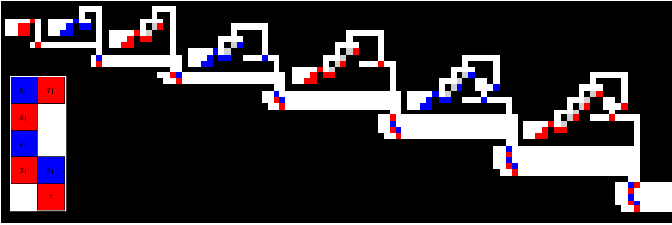
\includegraphics[width=0.45\textwidth]{fig1b1.pdf}%
  }  \\ \vspace{-.8em}
\subfloat[Same factory, 18 commanded moves, 136 unit steps\label{cw_25}]{%
  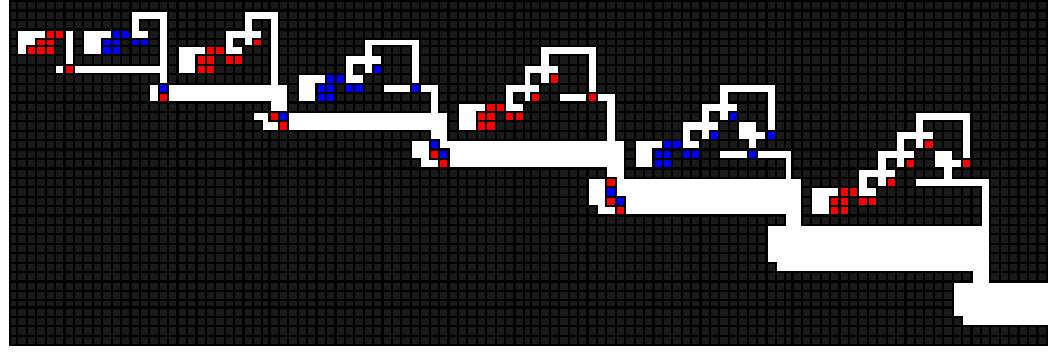
\includegraphics[width=0.45\textwidth]{fig1b1move18.pdf}%
  } \\ \vspace{-.8em}      
\subfloat[Parallel assembly with three factories, 28 commanded moves, 221 unit steps, three complete polyominoes\label{cw_50}]{%
  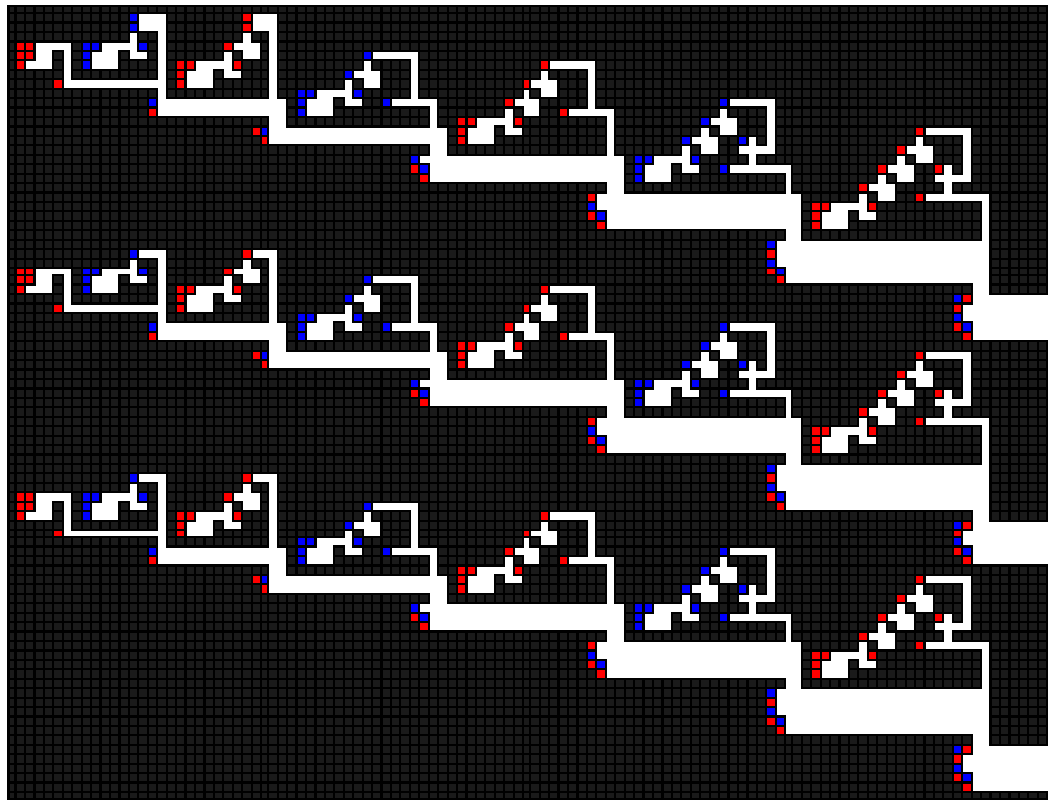
\includegraphics[width=0.45\textwidth]{fig1b1move28.pdf}%
  } 
\caption{\label{fig:factorySchematics}Factory schematics for assembling the seven-tile polyomino in (a).  Numbers and arrows on the polyomino show the build order and direction for build. All particles are actuated simultaneously by the same global field. Each factory is designed so at full production every clockwise control input sequence completes another polyomino.}
\end{figure}
 
Having only one global signal that uniformly affects all robots at once
limits the swarm's ability to perform complex operations.
Independent control is possible by designing heterogeneous particles that respond differently to the global input, but this approach requires precise differences in each particle and is best suited for small populations. 
Alternatively, control symmetry can be broken using interactions between the robot swarm and obstacles in the environment. 
This paper builds on the techniques for controlling many simple particles with uniform control inputs presented in \cite{Becker2013f,Becker2014,Becker2014a}, where
we demonstrated how such a system could  implement digital computation.
Fig.~\ref{fig:factorySchematics} illustrates the main contribution of this paper: algorithms to produce a factory that uses global inputs to assemble arbitrary polyominoes.

This paper combines microscale hybrid organic/inorganic particles with novel swarm control algorithms for mask-free programmable patterning and micro-assembly. 
Specifically, this paper applies swarm control and particle logic computations to magnetically actuate artificial cells, to use them as micro-scale robotic swarms that create complex, high resolution, 2D patterns and assemblies.

\paragraph{Microscale Biomanufacturing}
Naturally derived biomaterials as building blocks for functional materials and devices are increasingly desired because they are often environmentally and biologically safer than purely synthetic materials. 
One such class of materials, polysaccharide based hydrogels, are intriguing because they can reversibly encapsulate a variety of smaller components. Many groups have termed these loaded-alginate particles  \emph{artificial cells}, because they mimic the basic structure of living cells (membrane, cytoplasm, organelles, etc.) \cite{chang2005therapeutic,prakash2007artificial,chang2007artificial}. 
Construction with these micron-sized gels has numerous applications in industry, including cell manipulation, tissue engineering, and micro-particle assembly \cite{weibel2007microfabrication,abbott2007robotics,yi2006microfluidics,castillo2009manipulation,sitti2015biomedical}, but requires fundamental research in biology, medicine, and colloidal science. 
While there are several methods to efficiently fabricate these particulate systems, it is still challenging to construct larger composite materials out of these units~\cite{assal2015highlights}. Traditional methods of assembling larger macro-scale systems are unemployable due to the change of dominant forces at small length scales. 
In particular, forces due to electromagnetic interactions dominate gravitational forces at the micro-scale resulting in strong adhesion and sudden shifts in the position of microparts under atmospheric conditions. 
%Furthermore, analogs of basic macroscale robotic elements have not been suitably designed and commercialized. 
To form constructs out of microgels, groups have traditionally turned to non-robotic microfluidic systems that utilize a variety of actuation methods, including mechanical, optical, dielectrophoretic, acoustophoretic, and thermophoretic~\cite{desai2007engineering, chiou2005massively,shields2015microfluidic,augustsson2009decomplexing,vigolo2010thermophoresis}. 
While each of these methods has proven to be capable of manipulating biological cells, each method has significant drawbacks that limit their widespread application. 
For example, microscale mechanical, acoustophoretic, and thermophoretic manipulation methods use stimuli that can be potentially lethal to live cells~\cite{lin2012application}. 
Furthermore, most, if not all, of these techniques require expensive equipment and lack control schemes necessary to precisely manipulate large numbers of cells autonomously.

\paragraph{Control Swarms Using Only Global Signals}
 Micro- and nanorobotic systems are an exciting frontier in robotics, with potential impacts in the fields of manufacturing and medicine. 
Chemists, biologists, and roboticists have shown the ability to produce very large populations (10$^3$--10$^{14}$) of small scale (10$^{-9}$--10$^{-6}$ m) robots using a diverse array of materials and techniques~\cite{rubenstein2012kilobot,ou2013motion,chiang2011toward}. 
Untethered swarms of these tiny robots may be ideal for on-site construction of high-resolution macroscale materials and devices. 
While these new types of large-population, small-sized, robotic systems have many advantages over their larger-scale counterparts, they also present a set of unique challenges in terms of their control. 
Due to  current limitations in fabrication, micro- and nanorobots have little-to-no onboard computation, along with limited computation and communication ability~\cite{chiang2011toward, chowdhury2015controlling, donald2013planning}.  
These limitations make controlling swarms of these robots individually impractical. 
Thus, these robotic systems are often controlled by a uniform global external signal (e.g. chemical gradients, electric and magnetic fields), which makes motion planning for large robotic populations in tortuous environments difficult.
At the macro-scale, automated control of devices floating in water in ~\cite{mermoud2012real} and fluidic self assembly in~\cite{mastrangeli2014automated} were presented, but as stochastic processes that can be turned on and off by a global signal.
We recently demonstrated that obstacles present in the workspace can deterministically break the symmetry of approximately identical robotic swarms, enabling positional configuration of robots~\cite{becker2013massive}. 
 Given sufficient free space, a single obstacle is sufficient for positional control over $N$ particles.  
This method can be used to form complex assemblies out of large swarms of mobile microrobotic building blocks, using only a single global input signal.

\paragraph{Microrobot Based Microassembly}
The ability to create microrobots, and control algorithms capable of autonomous manipulation and assembly of small scale components into functional materials is currently a major manufacturing challenge~\cite{chang2005therapeutic}. 
%To address this challenge, teams of microrobotic systems must work together intelligently to coordinate manipulation tasks in novel environments. 
While several microrobots capable of performing simple manipulation and assembly tasks have been reported~\cite{prakash2007artificial,chang2007artificial,weibel2007microfabrication,abbott2007robotics,yi2006microfluidics,castillo2009manipulation}, few have shown the ability to pattern intricate designs or assemble complex multi-component parts. 
Recently, groups have begun to develop cell-safe magnetically-actuated microrobotic systems for cell patterning, yet their method is limited in that these systems are manually controlled, not automated, and suffer from low spatial resolution~\cite{tasoglu2014untethered,tasoglu2014guided}. 
For recent advances in automated micro-assembly, see~cite{seymour2016automated}, but these techniques focus on a set of micro manipulators assembling one component at a time.
%but they require improvement in success rate for complex assemblies and reduction in the computation time it takes to plan the assembly sequence.


\paragraph{Assembly Planning}
Algorithm techniques for optimizing assembly operations have a rich history, see review article~\cite{rashid2012review}.
Our paper determines if a polyomino has a feasible assembly sequence, similar to the planning in~\cite{Su2007}.





 
